\section{Scenario B: Email Digest}
In the Email Digest Scenario,
we will identify a batch of up to 100 ranked tweets per day per interest profile.
At a high level, these results should be relevant and novel;
timeliness is not important as long as the tweets were all posted on the previous day.

As shown in Fig.\ref{fig:Bsys}, our system for this scenario mainly contains four modules:

\begin{itemize}
\item \textbf{Data cleaning module:} We pre-process all tweets during evaluation period. And we simply filter tweets that do not contain any keywords for each interest profile, and the rest tweets are chosen as candidate tweet collection, which will accelerate identifying possible relevant tweets for each profile.

\item \textbf{Query expansion module:} As microblog retrieval suffers severely from the
vocabulary-mismatch problem (i.e. term overlap between query and tweet is relatively small). To tackle this issue, we leverage web-based query expansion method to improve retrieval performance. As is known to all, Google search is the dominant search engine in the majority countries over the world, which indexes billions\cite{arlington2008google} of web pages, so that users can search for the information they desire through the use of keywords and operators. Therefore, we take the interest profile as the keywords to search in Google with Google Search Engine API before the evalution period.

As the user interest profile offered by TREC 2016 are JSON-formatted structure and each profile includes four fields, topid, title, description and narrative.
Here we only use the topic keywords as our \emph{OriginQuery} since we utilize external web resource to depict the background information, noted as \emph{ExpansionQuery}.

We utilize the expanded query to represent the interest profile and then estimate the relevance between the query and tweets.

\item \textbf{Relevance ranking module:} Similar with Scenario A, we utilize the KL-divergence language model based retrieval method to measure the relevance between query and tweet.

\item \textbf{Novelty verfication module:} Once we obtain the ranked tweet list after relevance ranking, we adopt the novelty verfication module along with pushed tweet pool to pick up novel tweets.


In this module, there are two kinds of strategies to measure novelty between tweets: (1)Language model. The higher relevance score between tweets, the less novelty they are. (2)Simhash\cite{charikar2002similarity}, which is a popular method to handle web page redundancy. simhash is one where similiar items are hashed to similiar hash values and we can calculate the bitwise hamming distance between hash values. The closer hamming distance between two tweets is, the more similar they are. The simhash code is calculated as follow,

\begin{equation}
\label{equ:lm}
Sim_{code} = sign(\sum_{i=1 \in n} w_{i} c_{i})
\end{equation}
where $w_{i}$ is the weight of term $i$ and $c_{i}$ is the hash code of term $i$, $sign$ is symbol function that make positive to 1 and negative to 0 for every bit in code.

\end{itemize}

\begin{figure}[htbp]
\centering
{
	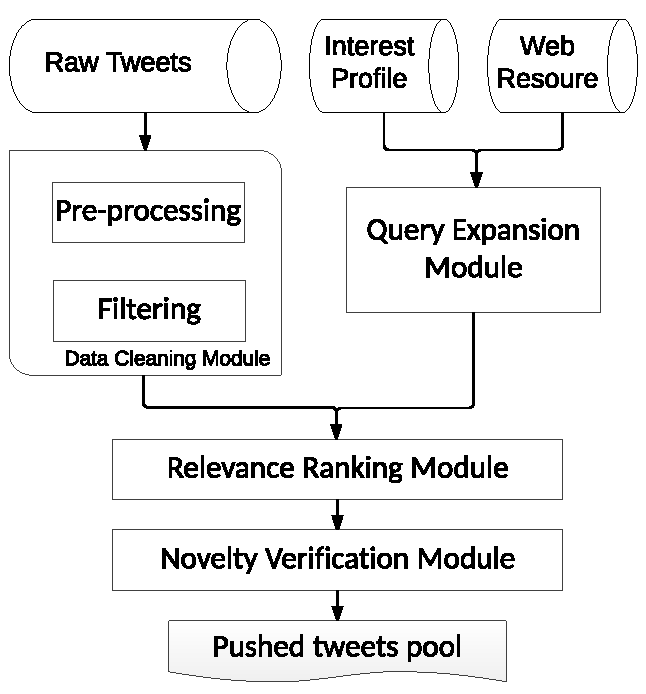
\epsfig{file=figures/b.pdf,width=0.45\textwidth}
}
\caption{Scenario B System Framework.}
\label{fig:Bsys}
\end{figure}


